% Chapter 6

\chapter{Feature Analysis} % Main chapter title

\label{Chapter6} % For referencing the chapter elsewhere, use \ref{Chapter6} 

\lhead{Chapter 6. \emph{Feature Analysis}} % This is for the header on each page - perhaps a shortened title

%----------------------------------------------------------------------------------------

To better understand the individual contributions of each feature used for email classification to the overall effectiveness of the classifier, we next present an analysis of the ability of each to capture information and its effect on the overall accuracy of the classifier.

\section{Comparison Between Naive Bayes and SVM Classifiers}
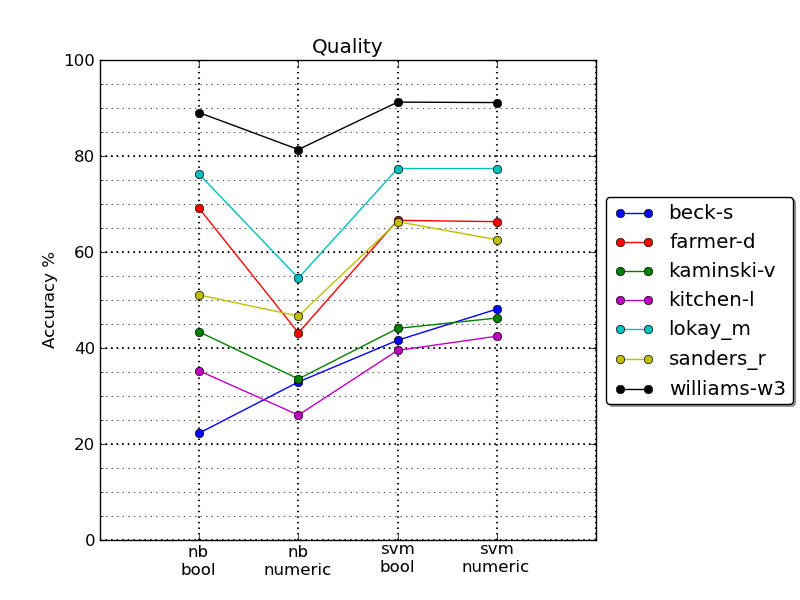
\includegraphics[width=15cm]{Quality.png}

\section{Tuning the Word Frequency Feature Threshold for Naive Bayes Using Boolean Attributes}
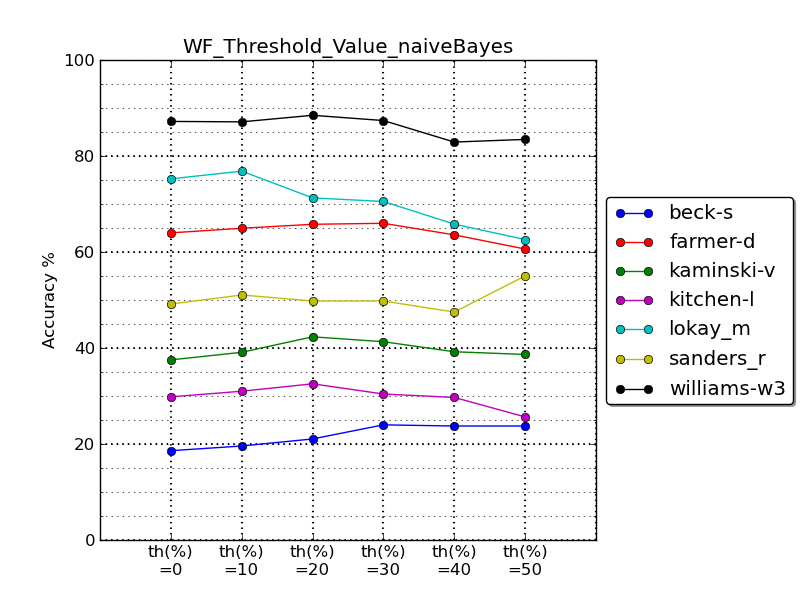
\includegraphics[width=15cm]{WF_Threshold_Value_naiveBayes_bool1.png}

\section{Tuning the Word Frequency Filter Threshold for SVM Using Boolean Attributes}
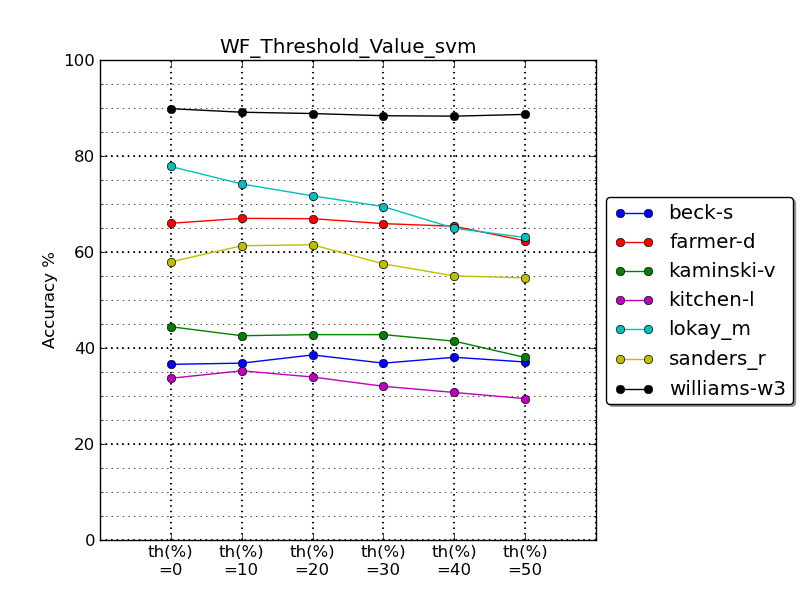
\includegraphics[width=15cm]{WF_Threshold_Value_svm_bool1.png}

\section{Tuning the Word Frequency Filter Threshold for SVM Using Numeric Attributes}
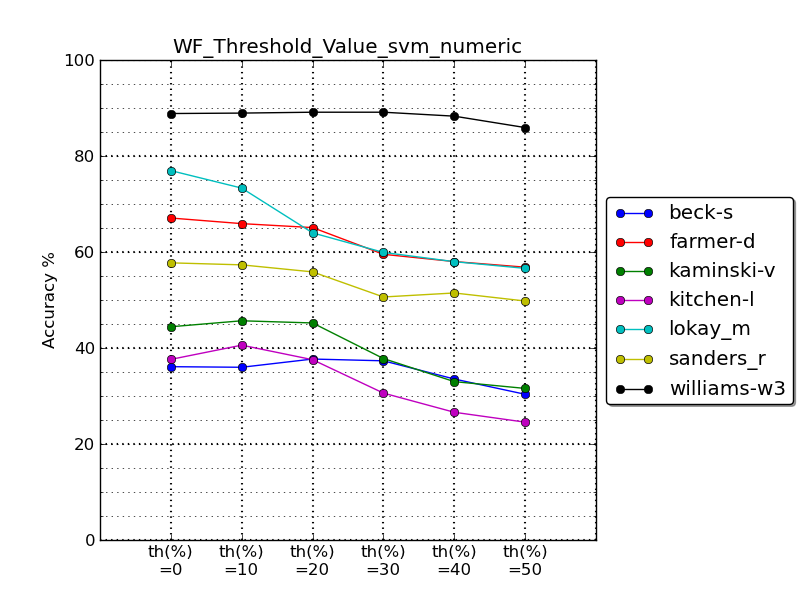
\includegraphics[width=15cm]{WF_Threshold_Value_svm_numeric.png}

\section{Combinations between sender/WF/Size/Subject features Using Naive Bayes}
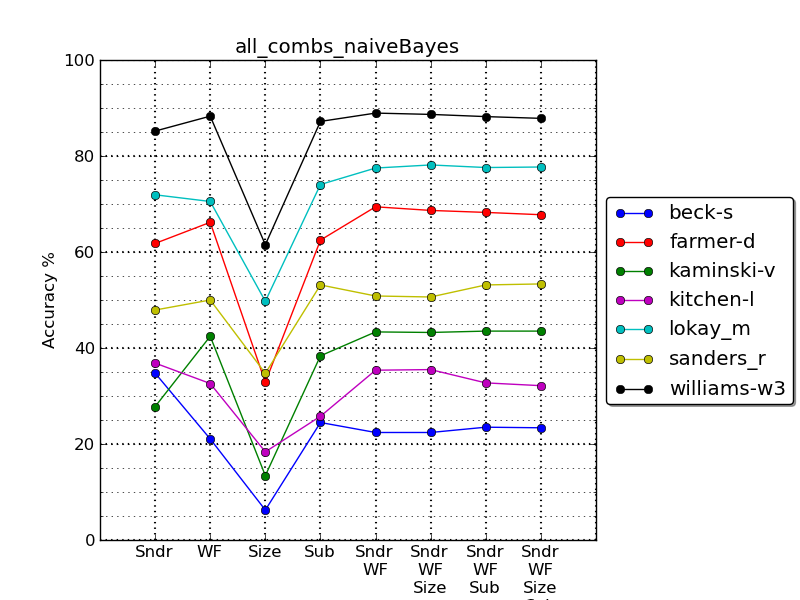
\includegraphics[width=15cm]{all_combs_naiveBayes.png}

\section{Combinations between sender/WF/Size/Subject features Using SVM}
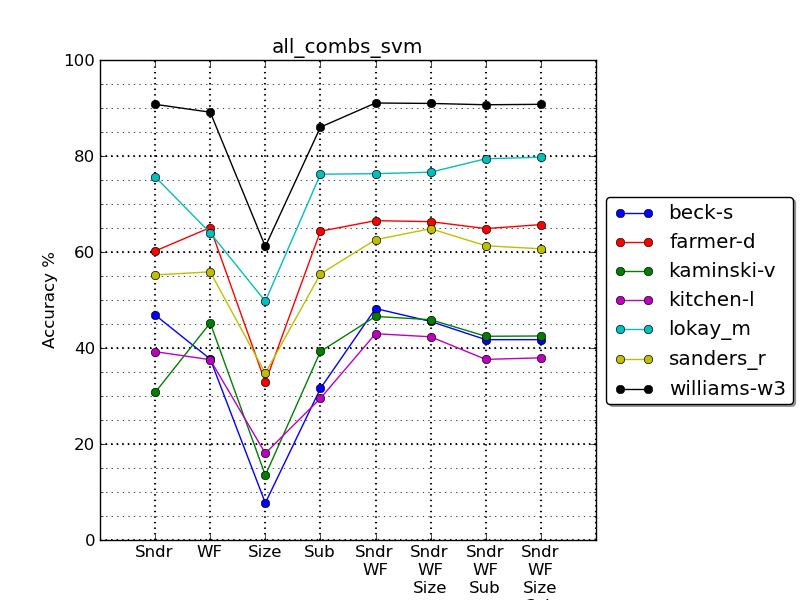
\includegraphics[width=15cm]{all_combs_svm.png}


\section{Feature Ranking}

\section{Conclusion}
\begin{itemize}
\item Using boolean attributes with NaiveBayes is better than using numeric attributes.
\item Using numeric attributes with SVM is better than using boolean attributes.
\item SVM outperforms NaiveBayes in almost all the cases.
\item Classification using the sender feature alone yields good results.
\item Best combination so far is using the sender feature along with the WordFrequency feature
\end{itemize}

Finally, formal tests and experiments will be conducted where more features and different combinations will be used. Also tuning the parameters of feature has a good impact on the results, so more experiments to select the best tunings should be carried out for each feature.

